%---------------------------------------------------------------------------------
\chapter{Numerical methods}
\label{chap:numerical-methods}
%---------------------------------------------------------------------------------
In real world problems, ODE systems are frequently used. A general form of an initial value problem is as follows: 
\begin{align}
    y'&=f(x,y)\\
    y(x_0) &= y_0
\end{align}
for $x \in [x_0, X_M]$. \\

Throughout the report, the following notation will be used:
\begin{itemize}
    \item $y_n$ - numerical approximation of $y(x_n)$
    \item $y(x_n)$ - analytical solution at mesh point $x_n$
    \item $x_n$ - mesh points of defined range, where
\end{itemize}

\begin{align}
    x_n &= x_0 + nh\\
    h &= \frac{(X_M - x_0)}{N}
\end{align}

for $n = 0,\dots, N$.

However, in general, these models cannot be solved analytically. Therefore, the solution has to be estimated by numerical methods. The most popular and simple method is the Euler's method.

Intuitively, the Euler's explicit method tries to estimate the value at the next step following the gradient of the solution at current point.

\section{One-step methods}
\label{sec:one-step-method}
The Euler's explicit method has the following definition,  
\begin{equation}
    y_{n+1} = y_n + hf(x_n,y_n)\\
\end{equation}
Starting from the initial value, the solution at the subsequent mesh point is estimated to follow a straight line with gradient as given.

The implementation is as follows:
\begin{lstlisting}[language=Python, caption= {Euler's explicit method}, title={Euler's explicit method}, label=Euler_explicit_code]
y_n = [self.initial_value]
x_n = [self.x_min]

# Calculate approximated solution for each mesh point.
for n in range(1, self.mesh_points + 1):
    step = [self.mesh_size * f for f in self.func(x_n[-1], y_n[-1])]
    y_n.append([a + b for a, b in zip(y_n[-1], step)])
    x_n.append(self.x_min + n * self.mesh_size)

return x_n, y_n
\end{lstlisting}

A vector of numerical solution and a vector of mesh points are initialised with their respective initial values. At each iteration, the mesh point and the numerical solution at the mesh point are calculated. The series of mesh points and its solution are returned.

The truncation error of the Euler's explicit method is defined to be the difference of exact solution with the numerical solution given the exact solution of previous mesh point is known. Therefore, we have that the truncation error for Euler's explicit method to be

\begin{equation}
\label{eqn:trun_err_def}
    T_n \defeq \frac{y(x_{n+1}) - y(x_{n})}{h} - f(x_n, y(x_n))
\end{equation}
According to Taylor's series expansion, we have 
\begin{equation}
    y(x_n + h) = y(x_n) + hy'(x_n) + \frac{1}{2}hy''(\xi_n)
\end{equation}
for $\xi_n \in (x_n, x_{n+1})$. Substitute this to the truncation error, noting that $f(x_n, y(x_n)) = y'(x_n)$, we get
\begin{equation}
    T_n = \frac{1}{2}hy''(\xi_n)
\end{equation}
Therefore, the truncation error for Euler's explicit method varies linearly with the step size.

An example model 
\begin{align}
\label{eqn:example_model}
    f(x,y) &= -y \\
    y(0) &= 1
\end{align}
for $x \in [0, 5]$ is used throughout the report to check that the implementation follows the theory. The analytical solution to this problem is $y = e^{-x}$. Some examples of the solution to the given model can be found here: \href{https://nbviewer.jupyter.org/github/FarmHJ/numerical-solver/blob/main/examples/solver_convergence.ipynb}{Example model notebook}

According to the computation of the software, the truncation error graph is shown below. It is observed that $\log |T_n|$ increases linearly with $\log h$, same as the theoretical prediction. 

\begin{figure}
    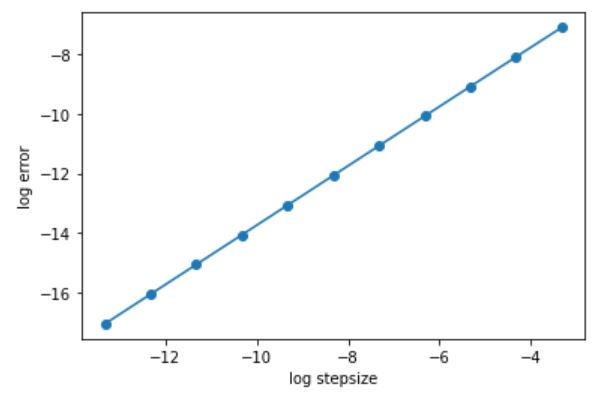
\includegraphics[width=0.95\columnwidth]{Euler_explicit_error_behaviour}
    \caption{Truncation error of Euler's explicit method for various step sizes.}
    \label{fig:Euler_explicit_error_behaviour}
\end{figure}

Other than the Euler's explicit method, the other one-step methods implemented are the Euler's implicit method, trapezium rule method and four-stage explicit Runge-Kutta method. The Euler's implicit method is defined to be
\begin{equation}
    y_{n+1} = y_n + hf(x_{n+1},y_{n+1}),\\
\end{equation}
while the trapezium rule method is
\begin{equation}
    y_{n+1} = y_n + \frac{1}{2}h[f(x_n,y_n) + f(x_{n+1},y_{n+1})].\\
\end{equation}
Using the same definition for truncation error in \ref{eqn:trun_err_def}, we have that the truncation error of Euler's implicit method and trapezium rule method are $T_n = -\frac{1}{2}hy''(\xi_n)$ for $\xi_n \in (x_n, x_{n+1})$ and $T_n = -\frac{1}{12}h^2y^{(3)}(\xi_n)$ for $\xi_n \in (x_n, x_{n+1})$ respectively.

When these methods are tested on the example model \ref{eqn:example_model}, the truncation error does not behave as expected, as shown in the graph below. This is probably due to the use of fixed point iteration algorithm to estimate the solution of implicit functions. The error of the fixed point iteration algorithm might be added to the error of the numerical method. Therefore, the difference of the numerical solution with the exact solution is larger for implicit methods as compared to Euler's explicit methods.

\begin{figure}
    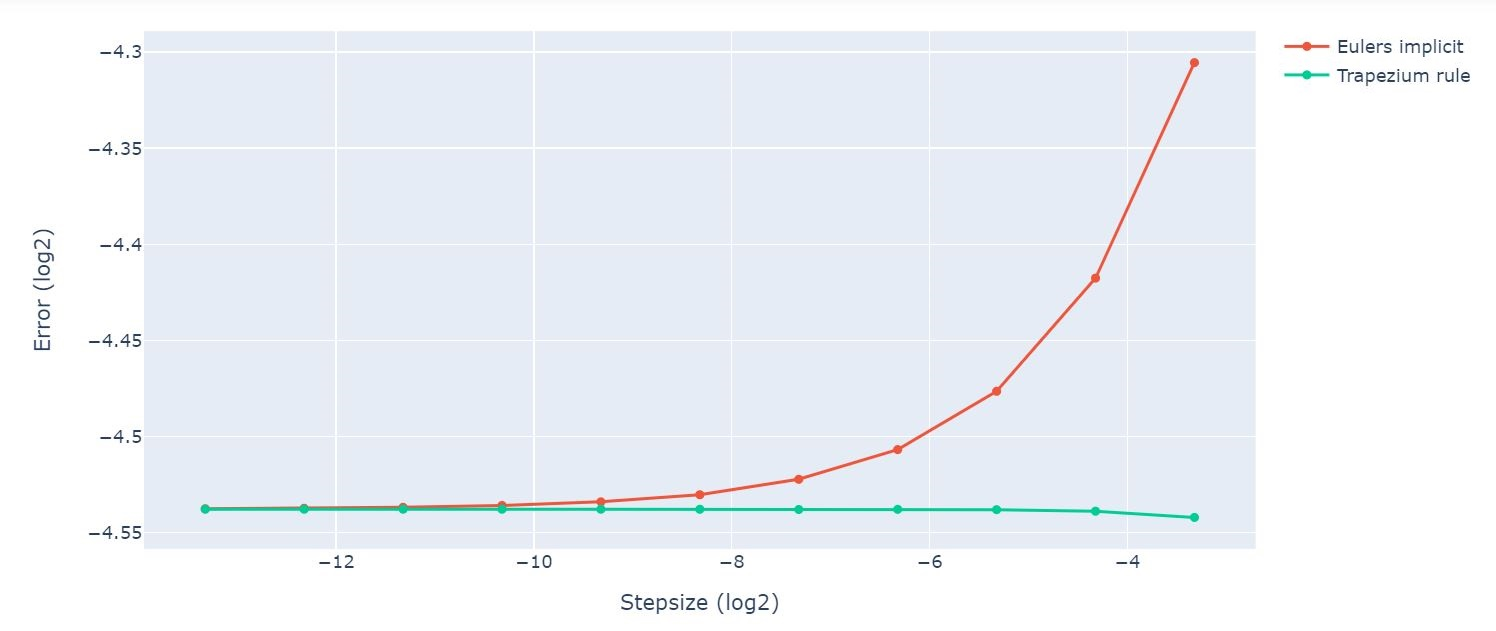
\includegraphics[width=0.95\columnwidth]{Eulerimplicit_trapezium_error_behaviour}
    \caption{Truncation error of Euler's implicit method and trapezium rule method for various step sizes.}
    \label{fig:Eulerimplicit_trapezium_error_behaviour}
\end{figure}

\section{Predictor-corrector methods}
\label{sec:predictor-corrector}
For the implicit one-step methods, numerical value at previous mesh point is chosen as the initial guess for the fixed point iteration algorithm. The predictor-corrector method suggests a more carefully chosen initial guess for the implicit methods. An explicit numerical method is used as a predictor for the initial guess of an implicit method. The initial value is then used for the iterations in the algorithm to solve an implicit function. The implicit method that refines the solution is known as the corrector method. 

The Euler-Trapezoidal method is a predictor-corrector that uses an Euler's explicit method as the predictor and trapezium rule method as the corrector. In this implementation, the trapezium rule method corrector is iterated until a set of conditions are satisfied. The conditions are set to be the difference between current iteration and previous iteration is lesser than a given threshold value or the number of iterations exceeds a certain amount. The figure below shows the graph of $\log |T_n|$ against $\log h$.

\begin{figure}
    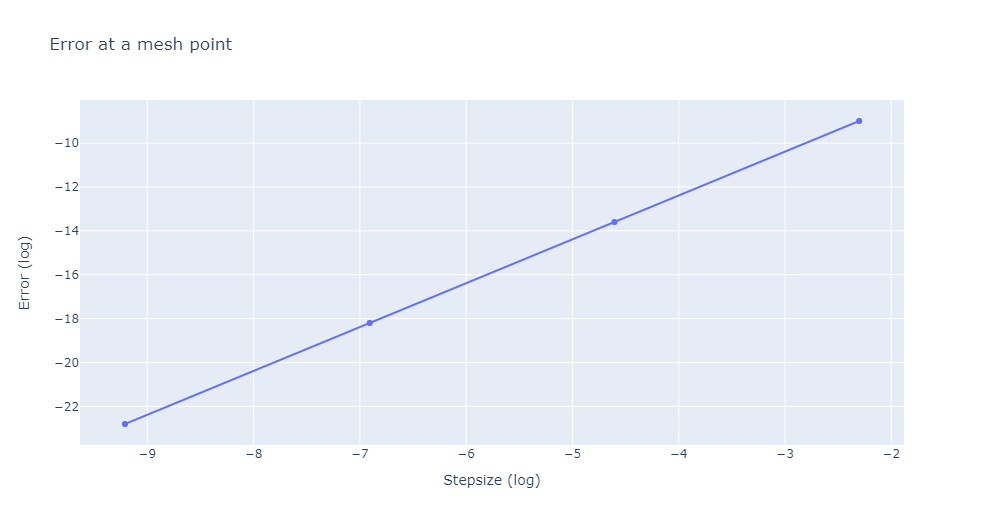
\includegraphics[width=0.95\columnwidth]{predictor_corrector_error_behaviour}
    \caption{Error of Euler-Trapezoidal method for various step sizes.}
    \label{fig:predictor_corrector_error_behaviour}
\end{figure}

\section{Adaptive method}
\label{sec:adaptive-method}
In some types of problem, the solution to the problem exhibits a behaviour where step sizes have to be sufficiently small for a stable solution. In other words, the solution have small changes with mesh points. Such problems are called stiff problems. In order to obtain a stable solution, the computational cost is high. Moreover, such stable solution would have resolutions higher than required for practical purposes.

The adaptive method focus on the achieving desired accuracy with low computational cost. The main idea of an adaptive method is to control the precision at each mesh point. The error at each mesh point is estimated. If the error is larger than a threshold value, a smaller step size is chosen. These steps are repeated until the error is smaller than the given threshold value.

The adaptive method implemented in this software is based on the BS23 (Bogacki and Shampine) and RKF45 (Runge-Kutta-Fehlberg) method. A lower order method is used to estimate the solution, while a higher order method is used to estimate the error. 

Absolute tolerance and relative tolerance were used in the implementation of the adaptive methods. Similarly, the implemented adaptive method is used to solve the example model \ref{eqn:example_model}. The adaptive methods were tested for convergence. Two comparisons were made, one based on absolute tolerance and the other on relative tolerance. As shown in the graph below, the error of the method is smaller for smaller tolerance, regardless of absolute tolerance or relative tolerance.

\begin{figure}
    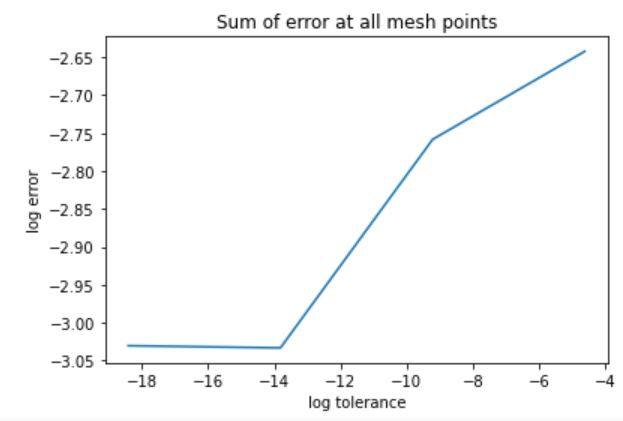
\includegraphics[width=0.95\columnwidth]{ode45_absolute_sum_error_behaviour}
    \caption{Total error of RKF45 method for various absolute tolerance.}
    \label{fig:ode45_absolute_sum_error_behaviour}
\end{figure}

\begin{figure}
    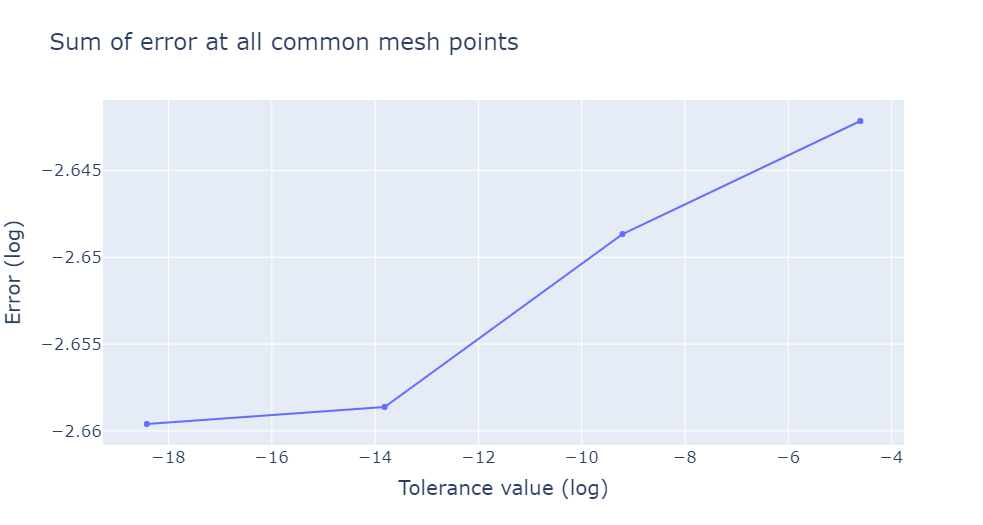
\includegraphics[width=0.95\columnwidth]{ode45_relative_sum_error_behaviour}
    \caption{Total error of RKF45 method for various relative tolerance.}
    \label{fig:ode45_relative_sum_error_behaviour}
\end{figure}